% latex pam-2.tex
% dvisvgm --no-fonts --exact --bbox=papersize --output=pam-2.svg pam-2.dvi
\documentclass[tikz,border=5pt]{standalone}
\usetikzlibrary{arrows.meta,decorations.pathreplacing}
\begin{document}
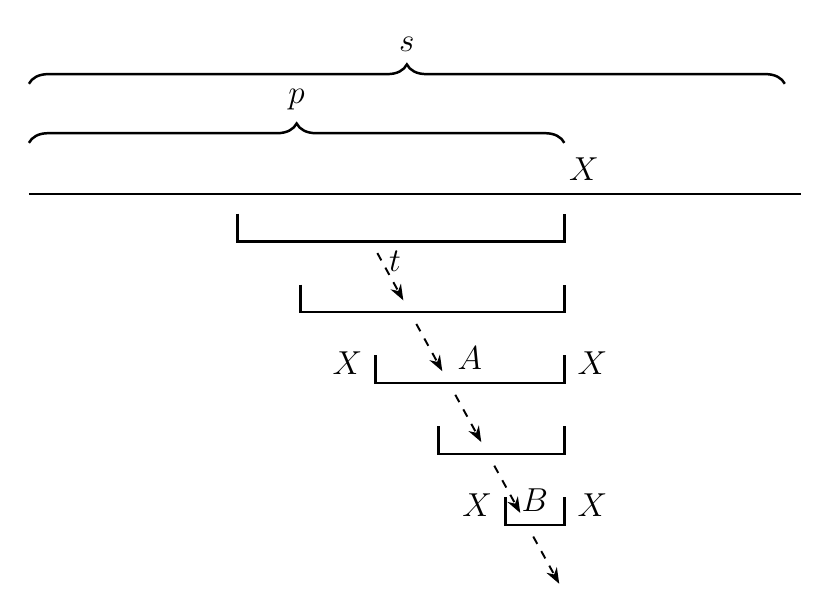
\begin{tikzpicture}[
    line width=0.9pt,
    font=\large,
    suffix/.style={dashed,-{Stealth[length=2mm]},line width=0.7pt},
    span/.style={decorate,decoration={brace,amplitude=7pt}}
  ]
  % p is the already processed prefix, and X is the appended character.
  \draw[span] (0,1.4) -- (9.6,1.4) node[midway,above=8pt] {$s$};
  \draw[span] (0,0.65) -- (6.8,0.65) node[midway,above=8pt] {$p$};
  \draw (0,0) -- (9.8,0);
  \node[above=1pt] at (7.05,0) {$X$};
  % All candidates are palindromic suffixes of p and share the right end.
  \draw (2.65,-0.25) -- (2.65,-0.6) -- (6.8,-0.6) -- (6.8,-0.25);
  \draw (3.45,-1.15) -- (3.45,-1.5) -- (6.8,-1.5) -- (6.8,-1.15);
  \node[above=1pt] at (4.65,-1.15) {$t$};
  \draw (4.4,-2.05) -- (4.4,-2.4) -- (6.8,-2.4) -- (6.8,-2.05);
  \node[above=1pt] at (5.6,-2.4) {$A$};
  \node[left=1pt] at (4.4,-2.15) {$X$};
  \node[right=1pt] at (6.8,-2.15) {$X$};
  \draw (5.2,-2.95) -- (5.2,-3.3) -- (6.8,-3.3) -- (6.8,-2.95);
  \draw (6.05,-3.85) -- (6.05,-4.2) -- (6.8,-4.2) -- (6.8,-3.85);
  \node[above=1pt] at (6.425,-4.2) {$B$};
  \node[left=1pt] at (6.05,-3.95) {$X$};
  \node[right=1pt] at (6.8,-3.95) {$X$};
  % Following suffix links finds A first, then B for the new fail link.
  % Every segment lies on x = 4.0125 - 0.55*y. The common diagonal
  % clears the left border of B while keeping all five arrows aligned.
  \foreach \y in {-0.75,-1.65,-2.55,-3.45,-4.35} {
    \draw[suffix] ({4.0125-0.55*\y},\y)
      -- ({4.0125-0.55*(\y-0.6)},{\y-0.6});
  }
\end{tikzpicture}
\end{document}
